\documentclass[12pt]{beamer}  
\usepackage{xeCJK}  
\usepackage{mathdots}  
\usepackage{graphicx}  
\usepackage{float}  
\usepackage{multirow}  
%\usepackage{cite}  
\usepackage{amsfonts, amsmath, mathrsfs, amsbsy, amssymb, dsfont,setspace}
\usepackage[square, comma, sort&compress, numbers]{natbib} 
\usepackage{algorithm}  
\usepackage{algorithmic} 
\usepackage{float} 
\usepackage{latexsym} 
%\usetheme{Warsaw}  
\usetheme{CambridgeUS}
\begin{document} 
\title{穿墙雷达成像}  
\author{黄臣}  
\date{\today}  
\frame{\titlepage}  
\begin{frame}
  \frametitle{DAS成像}
  由文献\citep{Tang2016Radar}\citep{Tivive2011An}可知,单基步进频率合成孔径雷达的成像方法
  可以采用Delay-and-Sum的beamforming.公式为:
  \begin{equation}
	y(n, m)=\sum_{p=0}^{P}\sigma_{p}\exp(-j2\pi f_{m}\tau_{n,p})
  \end{equation}
  其中$\sigma_{p}$为第$p$个目标的反射率,$\tau$为双程时延,因此位于第$(g,h)$像素点的复振幅为:
  \begin{equation}
	I(g, h)={1\over NM}\sum_{n=0}^{N-1}\sum_{m=0}^{M-1}y(n, m)\exp(j2\pi f_{m}\tau_{n,(g,h)})
  \end{equation}
\end{frame}
\begin{frame}
  \frametitle{真实实验场景描述}
  场景数据来自文献\citep{Dilsavor2005Experiments}所作出的实验。
  \begin{figure}
  \centering
  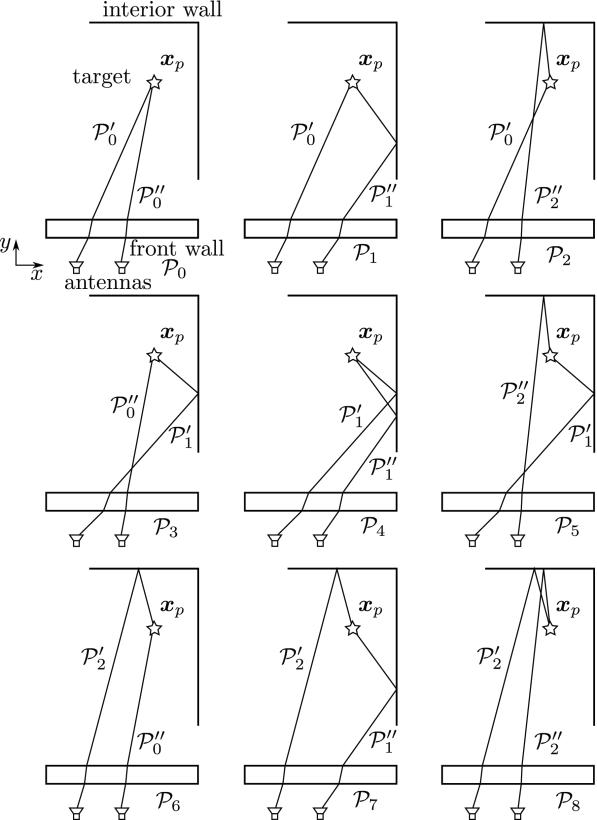
\includegraphics[width=0.6\textwidth]{fig2.jpg}
  \end{figure}
\end{frame}
\begin{frame}
  \frametitle{实验结果}
  文献\citep{Tivive2011An}中在有墙体反射情况下,直接成像的结果为:
  \begin{figure}
  \centering
  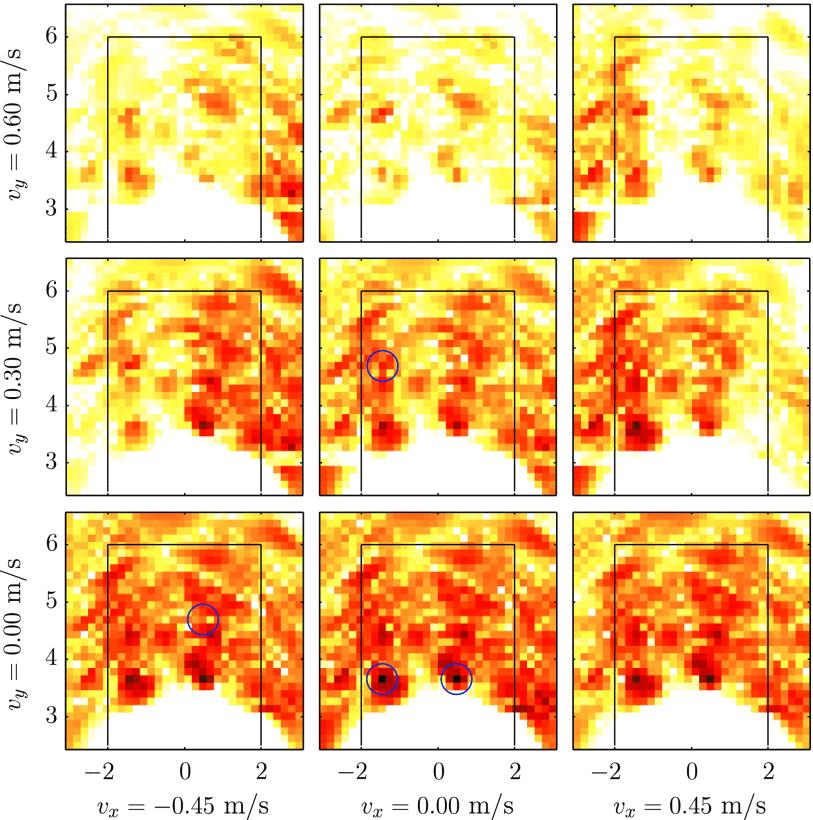
\includegraphics[width=0.9\textwidth]{fig4.jpg}
  \end{figure}
\end{frame}
\begin{frame}
  \frametitle{实验结果}
  \begin{columns}
  \footnotesize
	\begin{column}{0.5\textwidth}
	  无墙体干扰
  \begin{figure}
  \centering
  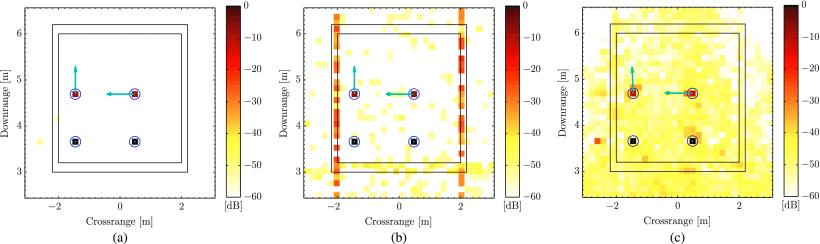
\includegraphics[width=0.65\textwidth]{fig5}
  \end{figure}
\end{column}
	\begin{column}{0.5\textwidth}
	  有墙体干扰:
  \begin{figure}
  \centering
  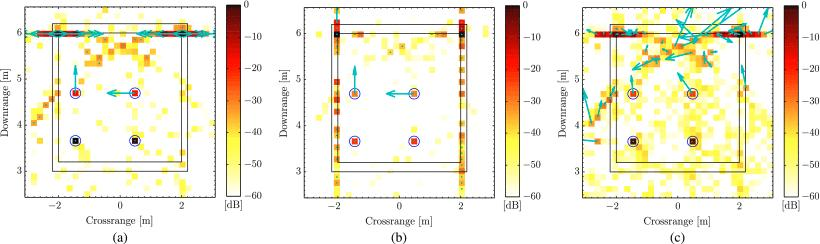
\includegraphics[width=0.65\textwidth]{fig6}
  \end{figure}
\end{column}
\end{columns}
\end{frame}
\begin{frame}
  \frametitle{压缩感知方法成像}
  文献\citep{Wang2017Look}给出了基于稀疏模型的贪婪算法,在HMP的基础上在迭代过程中
  嵌入了前瞻策略,以克服原子候选集中不可靠条目带来的误差。
  \par HMP简单说就是子空间追踪的每次索引选择时采用正交匹配追踪来实现,以
  保证基信号选择时的正交性。
  \par 而本文提出的LAHMP则是在HMP中加入在拓展集中通过对残差向量的范数
  意义上的最小化,来评估对未来恢复误差的影响,从而选择最佳索引的方法。
\end{frame}
\begin{frame}
  \frametitle{压缩感知方法成像}
  有墙体干扰场景下的成像结果为:
  \begin{figure}
  \centering
  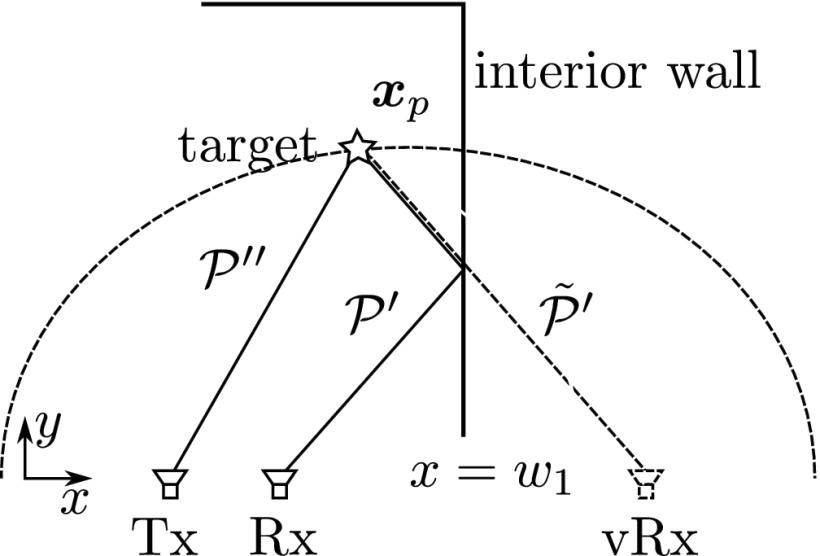
\includegraphics[width=0.9\textwidth]{fig3.jpg}
  \end{figure}
\end{frame}
\begin{frame}
  \frametitle{低秩方法去墙体回波}
  低秩矩阵逼近(LRMA)的方法被应用在很多地方,\citep{Ren2016Image}采用了一种
  加权核范数最小化的方法,用于先验盲图像去模糊。\citep{Tang2016Radar}则提
  出了一种迭代软阈值算法,用于使用减少的测量集来估计前墙回波的低秩矩阵和
  目标回波的稀疏矩阵。\citep{Bouzerdoum2017A}则是应用在了多极化信道的穿墙
  雷达成像上。\citep{Guo2018Low}则是指出在具有低秩结构的数据中,异常值和细小的密集
  噪声会污染数据,从而提出一种关于低秩矩阵恢复的稳健异常值估计方法。
\end{frame}
\begin{frame}
  \frametitle{低秩方法去墙体回波}
我们回波信号模型定为:
  \begin{equation} 
	\mathbf{Z}=\mathbf Z^{w}+\mathbf{Z}^{t}+\Upsilon.
  \end{equation}
  \par 所以我们的目标为估计$\mathbf{Z}^w$和$\mathbf{Z}^{t}$。文献\citep{Tang2016Radar}中采用了软阈值迭代的方法,优化模型可设置为:
\begin{equation}
\mathop\text{minimize}\limits_{\mathbf{Z}^{w},\mathbf{Z}^{t}} \Vert \mathbf{y}-\mathcal{A}(\mathbf{Z}^{w}+\mathbf{Z}^{t})\Vert_{2}+\lambda_{w}(\Vert \mathbf{Z}^{w}\Vert_{*}+\lambda\Vert \mathbf{WZ}^{t}\Vert_{1})
  \end{equation}
 使$\mathbf{Z}^w$的奇异值和矩阵$\mathbf{WZ}^t$的项收缩到0,阈值算子为:
  \begin{equation*}
	\mathcal{T}_{\tau}(x)=\frac{x}{\vert x\vert }(\vert x\vert -\tau)_{+}
  \end{equation*} 
\end{frame}
\begin{frame}
  \frametitle{低秩方法去墙体回波}
  文献\citep{Guo2018Low}则是指出核范数最小化往往需要付出昂贵的SVD代价,所以使用
  双线性因子分解来代替核范数最小化:
\begin{equation*} \| \mathbf {L}\|_{*} = \min _{ \mathbf {U}, \mathbf {V}}\frac {1}{2}\| \mathbf {U}\|_{F}^{2}+\frac {1}{2}\| \mathbf {V}\|_{F}^{2}\quad \mathop{\mathrm{s.t.}}\limits ~ \mathbf {L}= \mathbf {U} \mathbf {V}.\end{equation*}
其中$\mathop{\mathrm{rank}}\limits (\mathbf {L})=r\leq \min (m,n)$
并用$\mathbf{W}$表示噪声,用$\mathbf{\overline{W}}$表示离群点,
且$\mathbf {W}+\overline{\mathbf{W}}= \mathbf{1}$,最终公式为:
\begin{align*}&\min _{ \mathbf {U}, \mathbf {V}, \mathbf {W}}~\frac {1}{2}\| \mathbf {U}\|_{F}^{2}+\frac {1}{2}\| \mathbf {V}\|_{F}^{2}+\frac {\alpha }{2}\|\sqrt { \mathbf {W}}\odot (\mathbf {Y}- \mathbf {UV})\|_{F}^{2} \\&\hphantom {\min _{ \mathbf {U}, \mathbf {V}, \mathbf {W}}~}+\beta \|\overline { \mathbf {W}}\|_{1}+\gamma \sum _{i,j}(w_{ij}\log w_{ij}+\bar {w}_{ij}\log \bar {w}_{ij}) \\&\mathop{\mathrm{s.t.}}\limits ~ \mathbf {W}+\overline { \mathbf {W}}= \mathbf {1}; ~~ \mathbf {W} ~\text {and} ~\overline { \mathbf {W}}\in [{0,1}]^{m\times n},\tag{5}\end{align*}
\end{frame}
\begin{frame}{References}
 % \footnotesize
  \scriptsize
  \bibliographystyle{ieeetr} 
  \bibliography{ct.bib} 
\end{frame}
\end{document}
\begin{frame}
  \frametitle{Compressive Sensing Based Scene Reconstruction}
\end{frame}
\begin{frame}
  \frametitle{Compressive Sensing Based Scene Reconstruction}
\end{frame}
\begin{frame}
  \frametitle{Compressive Sensing Based Scene Reconstruction}
\end{frame}
